\documentclass{article}

% PACKAGES  
\usepackage[utf8]{inputenc}
\usepackage{amsbsy}
\usepackage{fixltx2e}
\usepackage{amsfonts}
\usepackage{natbib}
\usepackage{graphicx}
\usepackage{mathtools}
\usepackage{xcolor}
\usepackage{color} 
\usepackage{hyperref}
\usepackage{tcolorbox}
\usepackage{amsmath}
\usepackage{mathrsfs}
\usepackage{amssymb}
\usepackage{appendix}
\usepackage{amssymb}
\usepackage{amsthm}
\usepackage{fancyhdr}
\usepackage[T1]{fontenc}
\usepackage[colorinlistoftodos,prependcaption,textsize=tiny]{todonotes}
\usepackage[utf8]{inputenc}
\usepackage{lmodern}
\usepackage{minted}
\def\code#1{\texttt{#1}}
\usepackage{algorithm}
\usepackage{algpseudocode}
\usepackage[letterpaper,top=2cm,bottom=2cm,left=3cm,right=3cm,marginparwidth=2.0cm]{geometry}

\usepackage{pgfgantt}

% Theorem environments

\newtheorem{theorem}{Theorem}[section]
\newtheorem{corollary}{Corollary}[theorem]
\newtheorem{lemma}[theorem]{Lemma}
\newtheorem{definition}{Definition}
\newtheorem{example}{Example}
\newtheorem{remark}{Remark}


% Title page

\begin{document}
\hspace{95mm}\domark{Notes Prepared for M.Sc Thesis}

\section*{DT Algorithm}
These notes wrap up the final pieces of theory from the original paper on the Range Threshold Problem \cite{Gan2016}. Recall that so far we have introduced an algorithm that solves the \textit{restrained} RTS case of $m$ queries and a data stream of lenghth $n$ in time $O(n\log n + m\log m\log\tau_{max})$. Recall in the restrained case we restrict the problem so that $d=1$, all queries are preregistered, and $w(e_i) = 1$ for all stream elements $e_i$. \\
\\
We now cover how to remove each of these assumptions, and the consequences they have on runtime.


\subsubsection*{Supporting Dynamic Query Insertion}
As we have seen, the exisiting DT algorithm can handle Query deletion; by simply ignoring the corresponding Distributed Tracking instance, and then rebuilding the data structure whenever $m_{alive} < m$. To remove the prior assumption of all queries being pre-registered, we leverage the algorithmic technique of \textit{logarithmic rebuilding} \cite{BENTLEY1980301}. \\
\\
Logarithmic building is a well studied technique to convert an existing static data structure, into one that is \textit{semi-dynamic} in sense that the data structure can support \texttt{insert} operations. Referring to our appendix notes for this method, recall that it provides an additional logarithmic overhead to the total runtime to yield $O(n\log^2 m + m\log^2 m\log\tau_{max})$



\subsubsection*{Supporting $d>1$ Queries} 

As we initially defined, an RTS query specifies an axis-parallel query over a range $R = [x_1, y_1] \times \cdots \times [x_d, y_d]$. For an example as to how such a query could arise in practice, one can consider a stock tracker who may wish to register an RTS query of the form: 

\begin{center}
    \textit{``Alert me when $5,000$ shares of \texttt{AAPL} are traded between prices [300,305] \textbf{and} the Nasdaq trades between [3000,3050]''}
\end{center}
As it turns out, supporting higher dimensional queries is relatively straight forward, and can be done so through leveraging the central idea of multi-dimensional \textit{Range Trees} \cite{RTrees, DeBerg}. \\ 
\\
Similar to the techniques of a Range Tree we can support  $d>1$ dimensional queries by building and storing secondary subtrees at each internal node in our segment tree, with each successive tree adding a an extra logartihmic factor to both the run time and space per dimension. This brings our total runtime to $O(n\log^{d+1} m + m\log^{d+1} m\log\tau_{max})$ and space consumption to $O(m_{alive}\log^{d}m_{\alive})$

\begin{center}
    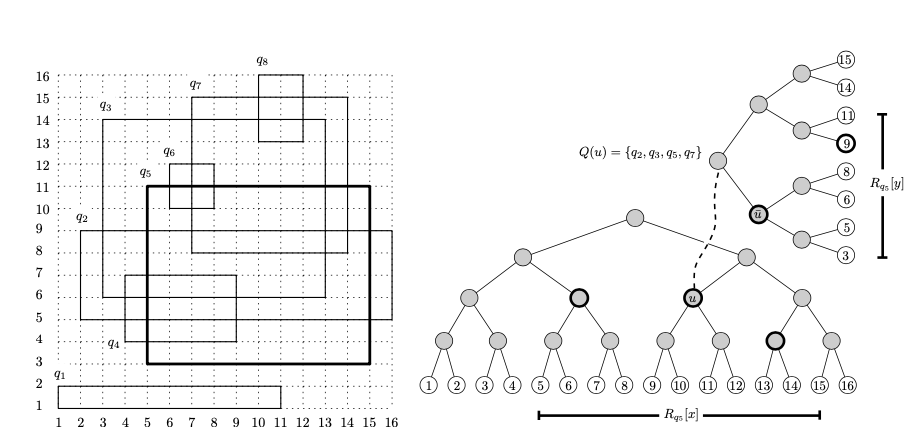
\includegraphics[scale=0.4]{images/rangetree.png}
\end{center}

\subsubsection*{Supporting Weighted Queries}
The final component to generalise is the support of queries on data streams where $w(e_t) \in \mathbb{N}_{\geq1}$. We won't extensively cover the details in these notes, but one can slightly modify the distributed tracking algorithm that is already discussed to solve this problem without any changes to the overall runtime. To make the modification, one slightly alters the number of message updates that are performed in the case of a large increase in a local counter. \\
\\
This leaves us with an algorithm that solves the general RTS problem in runtime $O(n\log^{d+1} m + m\log^{d+1} m\log\tau_{max})$ and space consumption to $O(m_{alive}\log^{d}m_{\alive})$






\newpage
\bibliographystyle{unsrt}%Used BibTeX style is unsrt
\bibliography{sample}

\end{document}
